\documentclass{deliverablereport}
\usepackage{wrapfig}

\deliverable{UI}{ipython-advanced-interacts}
\deliverydate{31/08/2018}
\duedate{31/08/2018 (M36)}
\author{Odile Bénassy and Nicolas M. Thiéry}

\begin{document}
\maketitle
% This will be the abstract, fetched from the github description
\githubissuedescription

\section{Introduction}

\TODO{Write a one (half) page summary of this introduction, and put it
  in the github description}

The \href{https://jupyter.org}{Jupyter Notebook} is a web application
that enables the creation and sharing of executable documents
containing live code, equations, visualizations and explanatory text.
Reaching far beyond the standard
\href{https://en.wikipedia.org/wiki/Read-eval-print_loop}{REPL}
interaction (Read-Eval-Print Loop), a key feature of Jupyter is its
\href{http://jupyter.org/widgets}{Interactive widgets} which enable
real time interactive data visualizations; the Jupyter community has
developed a large array of widgets for interactive 2D and 3D
visualization of data in the form of charts, maps, tables, etc; see
e.g. \delivref{UI}{vis3d} for ODK's contribution to 3D visualization.
Furthermore, widgets can be \emph{composed} to build rich
applications, with all the usual UI components (e.g. menus, sliders,
or layout control).

\begin{figure}[h]\begin{center}
  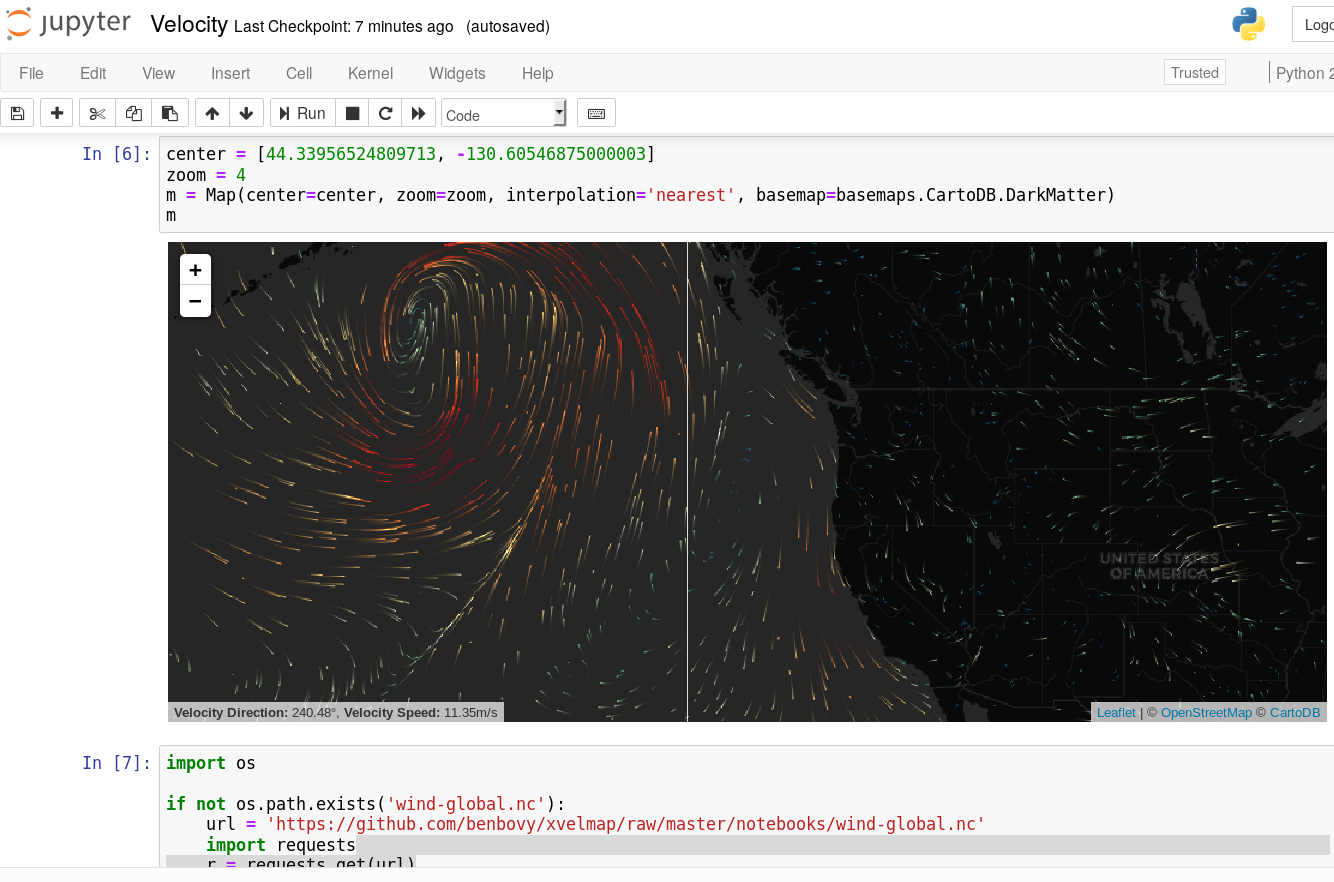
\includegraphics[width=\textwidth]{images/Velocity}
\end{center}\end{figure}

\TODO{screenshots: e.g. ipyleaflet + some application (exple appli web)}

\newpage

Hence, the Jupyter stack provides a very flexible environment catering
for use cases ranging from a novice users typing just a few commands
or browsing interactive documents to more advanced users authoring
rich interactive applications for their fellows.

The question we are tackling in this report is how this technology --
and specifically Jupyter widgets -- can be leveraged for pure
mathematics. The unique challenge comes from the huge variety of
mathematical objects that the user may want to visualize and
manipulate, some even coming with several natural ways to be
represented.

%\newpage

\begin{figure}[h]\begin{center}
    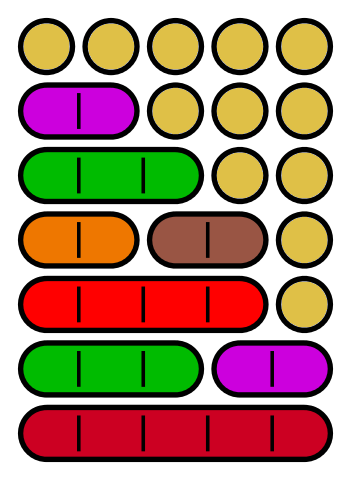
\includegraphics[width=0.20\textwidth]{images/partitions-of-5}
    \hspace{24px}
  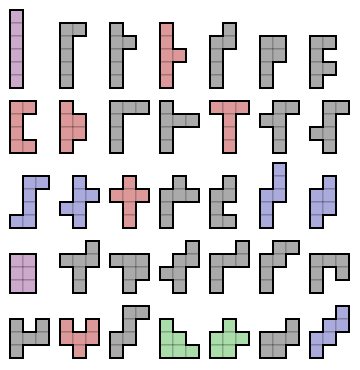
\includegraphics[width=0.25\textwidth]{images/hexominoes}
    \hspace{4px}
  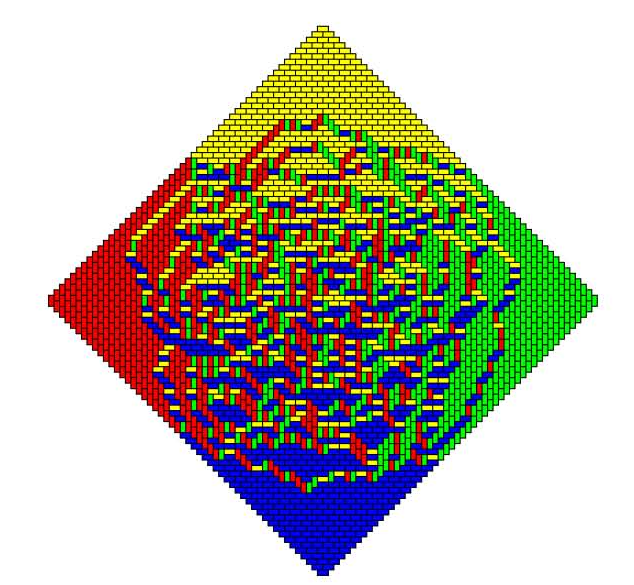
\includegraphics[width=0.36\textwidth]{images/AztecDiamond}
\end{center}\end{figure}\begin{figure}[h]\begin{center}
    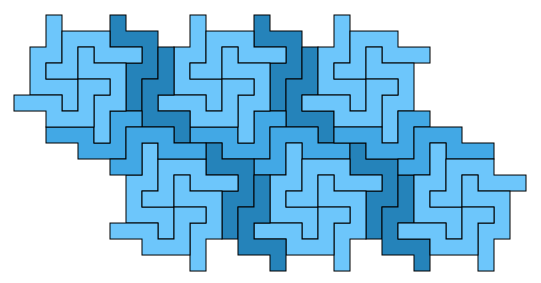
\includegraphics[width=0.4\textwidth]{images/nonominoes}
    \hspace{32px}
  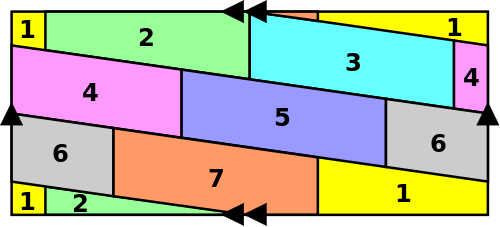
\includegraphics[width=0.4\textwidth]{images/500px-Torus_with_seven_colours}
\end{center}\end{figure}\begin{figure}[h]\begin{center}
  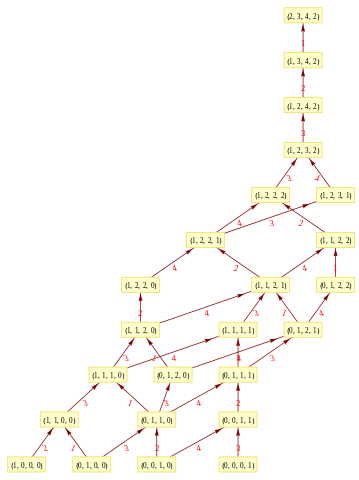
\includegraphics[width=0.3\textwidth]{images/359px-F4HassePoset}
    \hspace{4px}
  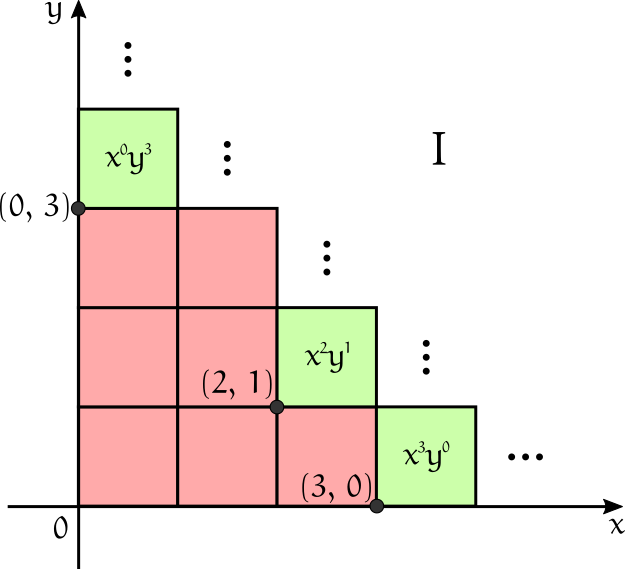
\includegraphics[width=0.3\textwidth]{images/Wikipic}
    \hspace{4px}
  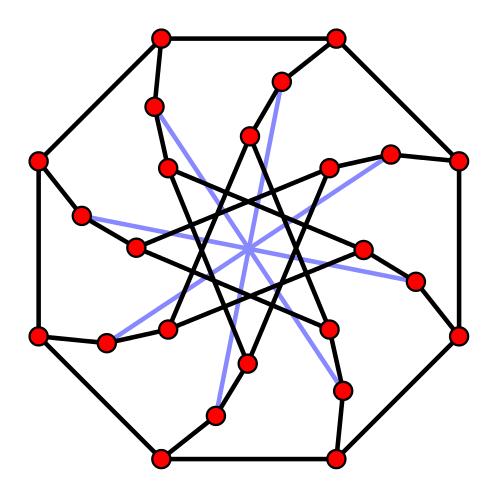
\includegraphics[width=0.3\textwidth]{images/500px-McGee_graph}
\end{center}\end{figure}\begin{figure}[h]\begin{center}
  
\includegraphics[width=0.3\textwidth]{images/fractioncont}
    \hspace{4px}
  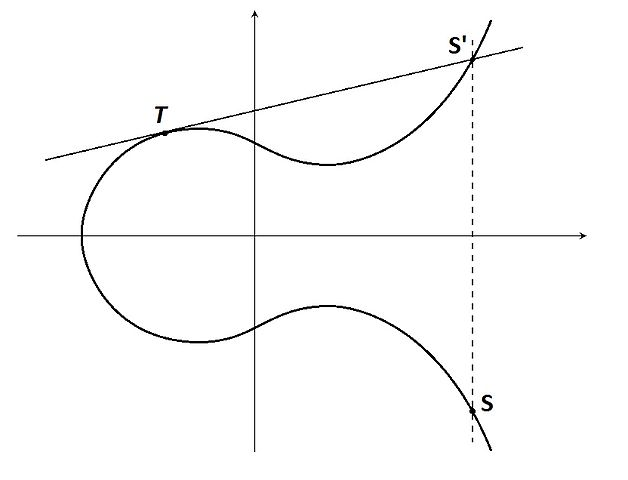
\includegraphics[width=0.3\textwidth]{images/elliptic-curve}
    \hspace{4px}
  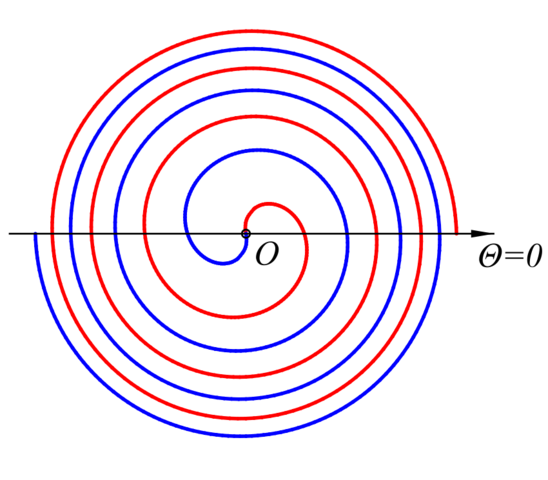
\includegraphics[width=0.3\textwidth]{images/548px-Fermat's_spiral_01}
\end{center}\end{figure}\begin{figure}[h]\begin{center}
  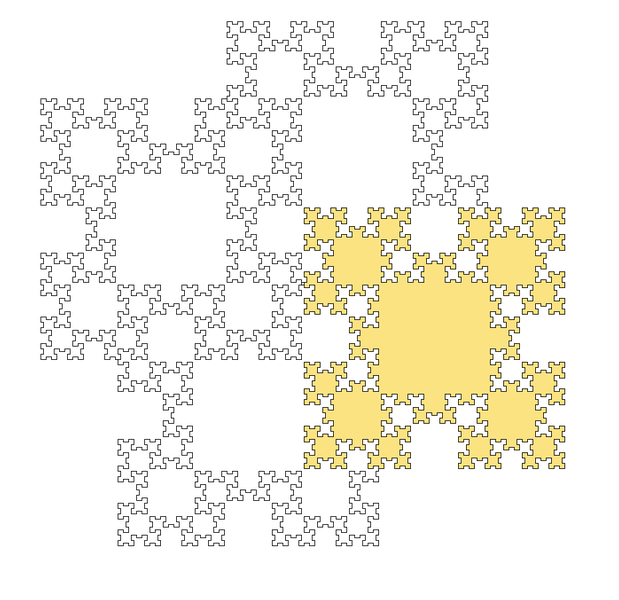
\includegraphics[width=0.3\textwidth]{images/619px-Tiling_Fibonacci_word_fractal}
    \hspace{32px}
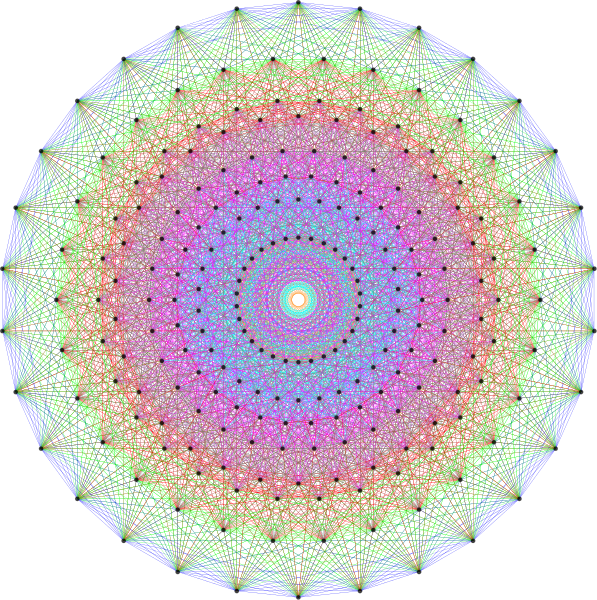
\includegraphics[width=0.3\textwidth]{images/597px-E8Petrie}
\end{center}\end{figure}

%\TODO{search on wikipedia for a nice collection of pictures: a
%  partition, a polyomino, an aztec diamond, a monomial ideal, a graph,
%  a poset, a formula - fraction continue, a curve, ...}. diagramme de Venn ; th des 4 couleurs sur une carte mathématique

\newpage

We therefore can't hope to provide hand crafted solutions for each
situation; instead we need to devise a toolbox of generic solutions
from which users can easily derive specialized visualizations for
their own pet objects.

We pursue two directions.

In the first one, we explore the development of widgets for the
graphical visualization of combinatorial objects.
The choice of this area of mathematics was, to some extent
out of personal interest and expertise, but more importantly because
devising good representations -- mental images -- of discrete objects
is at the heart of research in combinatorics. In Section~\ref{grid},
we report on the implementation in SageMath of a generic widget for
objects that admit a representation as a collection of cells on a 2D
grid, and specializations for typical objects such as partitions,
tableaux, polyominos, aztec diamonds, mazes.

\TODO{screenshot(s) of widgets displaying all of the above}

Another natural use case in combinatorics -- or more generally
discrete mathematics -- are objects that admit a graph-like
representation (trees, graphs, lattices of subgroups, crystals,
posets, discrete markov chains, to name a few). This use case is being
explored by the authors of the GAP package
\href{https://github.com/mcmartins/francy}{francy} under the
supervision(?) of ODK's member Markus Pfeiffer. Although ODK's
contribution in this direction is lightweight(?) at this stage, we
briefly report in Section~\ref{francy} on this use case to highlight
the lessons learned there and describe upcoming collaboration toward
bringing francy\'s features to SageMath.

In a second direction, we explore the use of Jupyter widgets not only
for the graphical visualization of an object, but for displaying a
page offering a synthetic overview of the information about that
object, including type, important properties and invariants, available
operations, related objects, documentation, etc. All sort of
information that is readily available by introspection but that a UI
can make easy to discover and emphasize according to relevance. The
challenge is that, given the huge variety of objects in a system like
SageMath, we can't afford to hand craft such pages for each type of
objects. In Section~\ref{sage-explorer} we report on our prototype
\lstinline{sage-explorer} that exploits the semantic embedded into the
system to produce a reasonable overview page automatically tailored to
each object.

\TODO{Screenshot of Sage-explorer?}

\TODO{Conclusion}

Altogether, the Jupyter Widget technology has proven as mature and
flexible as we hoped for. Designing new widgets does take some
expertise, but from the experience we gained, we are confident that it
lends itself well to the implementation of generic widgets by power
users that can be specialized by casual users and used by novices.

There remains two main challenges:
\begin{itemize}
\item How to best design widgets so that they can be reused across
  systems written in different languages? \TODO{Explain the tension
    kernel language / javascript}. \TODO{This will be explored by ... }
\item Widgets, as all modern web technologies, rely a lot on
  asynchronous execution. This is quite a different model from the
  Read-Eval-Print main loop that many not-so-young computational
  systems (including SageMath!) have originally been designed for, and
  such systems don't always behave well under asynchronous pressure:
  we have faced some bad crashes. How deep is the difficulty? How hard
  will it be to resolve it?
\end{itemize}

\section{State of the art}

\TODO{A standalone section? Or comments about it in the intro and along the way?}

In addition to the interactive widgets already delivered with ipywidgets (e.g. Sliders), numerous investigations, towards these goals, have been conducted in mathematical environments.

\begin{itemize}
\item The \href{http://www.lmfdb.org/}{LFMDB} database displays a comprehensive view of L-functions and Modular Forms in a web browser, yet misses manipulation possibilities on the objects.
\item In the \href{https://core.ac.uk/download/pdf/9839511.pdf}{The
  Larch Environment} document (2013), Geoffrey W. French presents his own graphical
  interactive programming environment called \emph{larch}.
  One of his main ideas is to
  \emph{coerce} objects into graphical representations. Meaning that
  every object must know how it can be graphically represented, this
  representation being the default one and can be tailored by the
  user: G.W. French speaks of different \emph{perspectives} for the
  same object. The Larch Environment also maintains a state of objects
  in order to automatically refresh the representation.
  However, the Larch environment is designed to run locally, i.e. not
  within any browser, and the project was discontinued in 2014.
\item Already within
  \href{http://mupad-combinat.sourceforge.net}{MuPAD-Combinat} project
  (2003-2004), an API was developed for a graphical representation
  combinatorial objects and their properties ; see
  \href{http://mupad-combinat.sourceforge.net/doc/en/Cat_Combinat/CombinatorialClassWith2DBoxedRepresentation.html}{Combinatorial
    Class With 2DBoxedRepresentation}. Yet this representation was
  limited to text-graphics i.e. ``ASCII art''.
\end{itemize}


\section{A generic widget for objects with a grid-like representation}
\label{grid}

\subsection{A generic grid view widget}

\begin{wrapfigure}{r}{0.25\textwidth}
    \begin{center}
      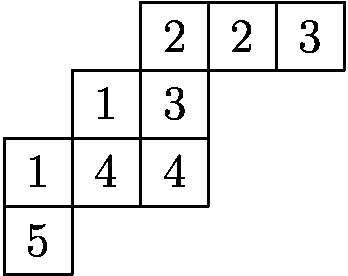
\includegraphics[width=100px]{images/JDTSlide}
      %\caption{A grid widget}
\end{center}
\end{wrapfigure}

We decided to first implement a generic widget meant for all SAGE-objects that can
be grid-like represented, i.e. all objects that can be described by
filling out some of the boxes in a 2-dimensional grid.

For example a skew tableau:

This use case combined several advantages:
\begin{itemize}
\item The UI part was relatively straightforward, for example
  requiring no Javascript side extension;
\item Little mathematical background was required; this, together with
  the previous point, made for a smooth learning curve for our
  Research Software Engineer;
\item It was a low hanging fruit with a large coverage;
\item The end result is immediately useful to colleagues, enabling
  early feedback from users;
\item There is a large variety of potential specializations, each with
  it's own quirks and specifics.
\end{itemize}
Hence, this use case provided a unique challenge: all the difficulty
resided in the the design of a generic solution that encapsulates as
much of the technicalities as possible, enabling users to specialize
the generic solution for their own pet objects with little expertise.

\subsection{Description of the design, of the API that subclasses must
  implement, code examples}

This widget, called \emph{GridViewWidget}, implements the following:

\begin{itemize}
 \item loading an object and calculating its cells positions and
   contents
 \item getting/setting this object
 \item editing a cell
 \item adding/removing cells
 \item after a change, checking the new object type
\end{itemize}

\emph{GridViewWidget} is subclassed to \emph{TileGridWidget} class,
which implements the actual grid-like display with one tile for each
object cell.

The users can specify their own tile shape. For example they can
use \emph{IPyWidgets} buttons or text inputs.

\subsection{Potential applications}

\begin{wrapfigure}{r}{0.25\textwidth}
    \begin{center}
      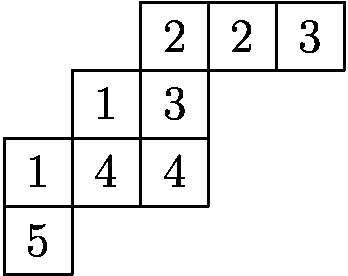
\includegraphics[width=100px]{images/JDTSlide}
      %\caption{A tableau widget}
\end{center}
\end{wrapfigure}

Grid-like representable objects cover many algebraic or combinatoric
objects: matrices, graphs, tableaus, skew tableaus, ribbons ..

Apart from displaying and editing an object, more possibilities can be
imagined

\TODO{imagination}

\begin{wrapfigure}{r}{0.25\textwidth}
    \begin{center}
      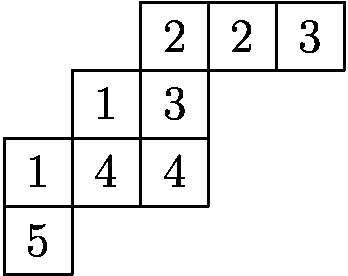
\includegraphics[width=100px]{images/JDTSlide}
      %\caption{A tableau widget}
\end{center}
\end{wrapfigure}

As an example, we have developed a domino-like representation of
\emph{grid-graph matchings} with a \emph{flipping} feature on neighboring dominos.

\TODO{an image with dominos in an Aztec Diamond}

The code is distributed as a Sage package
\href{https://github.com/sagemath/sage-combinat-widgets/}{sage-combinat-widgets}
which is meant to grow beyond this initial seed, attracting
contributions from the community, and presumably be integrated
progressively into SageMath.

\subsection{Strategy to get feedback from users}

\begin{itemize}
  \item Attending local seminars at \emph{Laboratoire de Recherche Informatique} or/and \emph{\href{https://www.lix.polytechnique.fr/}{Laboratoire d'Informatique de l'École Polytechnique}}
  \item Release some implementation examples for a few object types ; write a tutorial on how to write your own ; invite users to write feedback, either on the development mailing list, or on the  project \emph{sage-combinat-widgets} issues interface
  \item Take advantage on the next SAGE-days to organize a dedicated workshop and collect direct feedback there
\end{itemize}

\section{francy: an Interactive Discrete Mathematics Framework for GAP}
\label{francy}

\subsection{Description of Francy: features, devs, ...}

Francy framework enables building applications within Jupyter cells,
or in a web browser.

Mathematical objects are displayed in a very natural, graphical mode,
and support interactions such as moving graph nodes. A menu is also
displayed, mainly for activating/deactivating interactions.

Francy uses \href{d3js.org}{D3JS javascript library} to manipulate the
browser DOM for the graphical display itself.

Through its browser-loaded javascript code, francy calls a GAP engine to
intepret GAP code, then passes JSON data to D3JS.

\subsection{Francy is meant to become kernel-agnostic}

What francy does with GAP could be done also for any language. JSON
syntax would hold its language-agnostic data representation.

\TODO{How we plan to collaborate}

\section{Sage-explorer}
\label{sage-explorer}

\TODO{tension SAGE/javascript concernant l'emplacement des appels de
  méthodes}

\subsection{Sage-explorer should be as rich as LMFDB, and is interactive}

\TODO{Screenshot of http://www.lmfdb.org/EllipticCurve/Q/11/a/2}
\TODO{Comparative screenshot of the same curve in sage-explorer}

\TODO{A bunch of screenshots}

\subsection{Overview}

Sage-explorer is a container widget that comprises:

\begin{itemize}
  \item A block made of a title and a list of properties for the object
  \item A graphical representation of the object
  \item A list of object methods
  \item A panel for documentation and computations
\end{itemize}

\TODO{Illustration des zones}

\subsection{Object Properties}

The title block displays an object-identifying \emph{title}, its
\emph{category} and a list of its \emph{properties}.

Actually, there is no concept of \emph{property} in itself in Sage.

Yet some of the Sage object methods return a piece of information that
can be considered as \emph{properties}. Such as a the degree for a
polynomial degree, the dimension for a curve, or whether a graph is
planar or has loops ..

The fact, for a method result, to be possibly considered as a property
is in itself a piece of semantic information that can be stored in a
configuration file (which is the case with current published version),
or can be stored in the Sage code itself (which will in a way or
another most probably be the adopted solution in the future). See~\ref{semantics}

\subsection{Object Graphical Representation}
\label{representation}

The Sage explorer looks for any ``natural'' way of representing the
object graphically.

For a curve, or any mathplot-plottable object, there is already such a
``natural'' response.

For others, we try to use the work done in the
\emph{sage-combinat-widget} project.

As for properties (see above), the name of the widget class for an
object graphical representation is a piece of semantic information,
currently stored in the Sage-explorer configuration file, later very
possibly in the Sage source code itself (see \ref{semantics}).

The object graphical representation is meant to be responsive to some
actions on the object, such as highlighting elements, adding nodes ..

These interactions are not currently implemented in the library widgets but
this will be one of our high priority task in the next future.

\subsection{Object Methods}

The core of Sage explorer features is its list of methods.

All these methods are presented as menu entries, and dispatched in the
object parent class hierarchy, depending from
which class they get their definition.

\subsection{Object Documentation}

Within the main zone, a tab is dedicated to displaying documentation.

When no method is selected, it displays the documentation for the object itself.

When a method is selected, it displays the method documentation.

\subsection{Computations}

Within the main zone, a tab is dedicated to computations.

This tab is empty when no method is selected.

As soon as a method is selected, boxes appear, one for each method
argument (following the method signature and with names matching those
in the displayed documentation).

The user is invited to fill the boxes and then to press the
\emph{Run!} button. The explorer then calls Sage kernel to do the
computation and displays the result below the arguments boxes.

In a near future, some of the computation results will be graphically
displayed as well - on the widget. See \ref{representation}

\TODO{Description of how the page is built}

\subsection{Navigation}

Numerous links to new Sage objects appear in various explorer zones,
especially in properties and in method results.

Clicking on any link opens a new Explorer, for a new object.

A history is kept, in order to enable going back to the previous object.

An index page is also provided, displaying various lists of Python
categories to click on.

\subsection{Configuration and semantics}
\label{semantics}

Three configuration files specify:

\begin{itemize}
\item Graphical display widgets associated to Sage objects
  \item Properties associated to Sage objects, i.e. which object methods are
    to be considered as object properties.
\item The objects lists (or \emph{catalogs}) for the Explorer Index
\end{itemize}

To specify these, especially the first two, a set of logical rules
have been defined, are implemented in YAML syntax and parsed by the
Sage-explorer code.

In the future, we expect to get all this semantic information, or part of it,
written directly in Sage source code.

This could take the form of \emph{private attributes} or \emph{annotations}, like:

\begin{itemize}
\item a \emph{\_widget\_} attribute specified in Sage categories source files
\item specific annotations, using \emph{@} Python syntax for annotations
  \end{itemize}

Where will still remain, for the user, the possibility of overloading
the widget class - \emph{\_widget\_} being only the default) and
specify which of the \emph{properties} she wants to get rendered in effect.

Hence, there will be a contiuum between semantic written in Sage
source code and configuration files, taking into account semantic
information, logical rules specifying how to read this semantics, and
parametrization by the user, given that (for \emph{properties}:

\begin{itemize}
\item some semantics can be specified as object attributes: ``is this method a
  property?'' and
  \item ``is this property worth rendering by default?''  while we
    still have to decide
  \item ``is computing this property not going to slow down the display?''
\end{itemize}

\subsection{Upcoming work}

\begin{itemize}
\item develop interactivity for some methods in the widgets
\item tutorial: how to build a widget
\item enhance explorer index
\end{itemize}

\subsection{Strategy to get feedback from users?}

\TODO{See above (ou bien on recopie dès que c'est bien fixé)}

\appendix

\TODO{The demo notebooks?}



\end{document}

%%% Local Variables:
%%% mode: latex
%%% TeX-master: t
%%% End:

